\documentclass[oneside]{htwg-report}

% Use german umlaute
\usepackage{german,ngerman}
\usepackage[T1]{fontenc}
\usepackage[utf8]{inputenc}
\usepackage[ngerman]{babel}
\usepackage[autostyle=true,german=quotes]{csquotes}

%\usepackage[table]{xcolor}\usepackage{float}
%\usepackage{xcolor,colortbl}

\addbibresource{./bib/report.bib}

\begin{document}

\pagenumbering{gobble}

%% 'reporttype' add background elements to the cover / front page
%% possible values are:
%% bachelor	--> B S C
%% master	--> M S C
%% other		--> none
\reporttype{master}

\reporttypetext{Teamproject (Master 3. semester)}

\newcommand{\verfasserA}{Simon Christofzik}
\newcommand{\verfasserB}{Paul Sutter}
\newcommand{\verfasserC}{Till Reitlinger}
\newcommand{\thema}{DeepRain: Rain forecast with neural networks and the visualization of these in an App}
\newcommand{\hoschschule}{HTWG Konstanz - University of Applied Sciences}
\newcommand{\institut}{HTWG Konstanz - Institute for Optical Systems}
\newcommand{\prueferA}{Prof. Dr. Oliver Dürr}


\title[Teamprojektthema]{\thema}

\doclocation{Konstanz}
\docdate{10. September 2020}

\makecover[]

\chapter*{Extended Abstract}

\begin{center}
	\begingroup
	\renewcommand*{\arraystretch}{1}
	\rowcolors{2}{white}{white}
	{\makeatletter	
		\begin{tabular}{p{3.2cm}p{9.6cm}}
			Topic: & \thema \\
			& \\
			Team members: & \verfasserA, \verfasserB, \verfasserC \\
			& \\
			Advisor: & \hoschschule \newline \institut \newline \prueferA \\
			& \\
		\end{tabular}
		
		\makeatother}
	\endgroup
\end{center}

\bigskip

In this Paper we try to predict precipitation for a range of 35 minutes in an area around Constance.
Therefore we are using machine learning techniques and train a UNet on radar data images. 
Here we present the result of precipitation prediction as well with regression as with classification. 
Both approaches provide good results. Source code and full length documentation in german can be found at GitHub: \url{https://github.com/thgnaedi/DeepRain}.


\printbibliography[title={References}, heading=subbibliography]


\twocolumn
\section*{Introduction}

\begin{sloppypar}
\tolerance 9999
Even today, rain forecasts are still very computationally complex and relatively inaccurate. 
Therefore, it may make sense to make such predictions with the help of neural networks. 
These do not require as much computing power and can recognize a pattern in the often chaotic data even without complex physical models.
\end{sloppypar}

\section*{Data}

\section*{Data preprocessing}

\begin{figure}[ht]
\centering
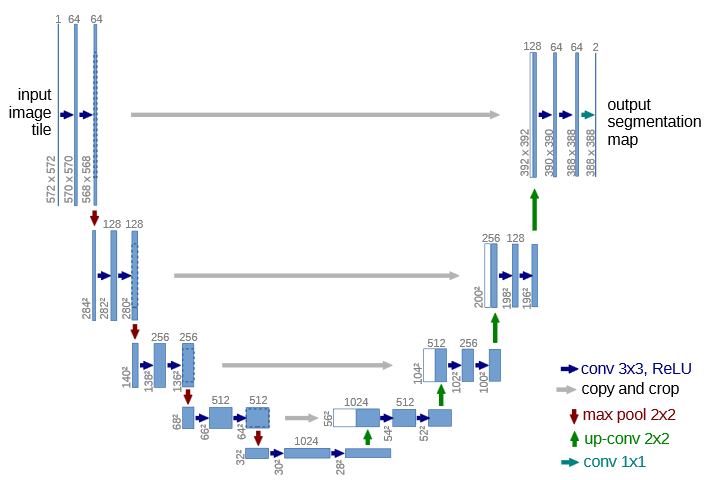
\includegraphics[width=0.8\linewidth]{../pics/UNet_Biomedical}
\caption{The image is taken from the university of Freiburg~\cite{ronneberger2015u}}
\end{figure}

\begin{sloppypar}
\tolerance 9999
\noindent
\end{sloppypar}

\section*{DeepRain Application}

\begin{figure}[ht]
    \centering
    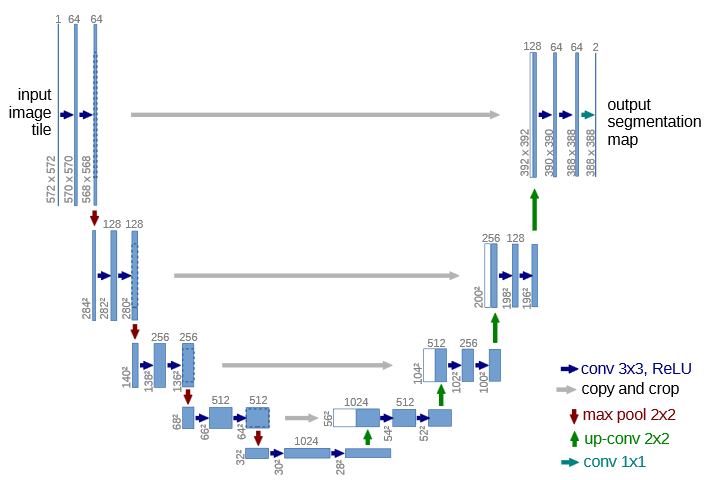
\includegraphics[width=0.8\linewidth]{../pics/UNet_Biomedical}
    \caption{The image is taken from the university of Freiburg~\cite{ronneberger2015u}}
\end{figure}


\begin{figure}[ht]
    \centering
    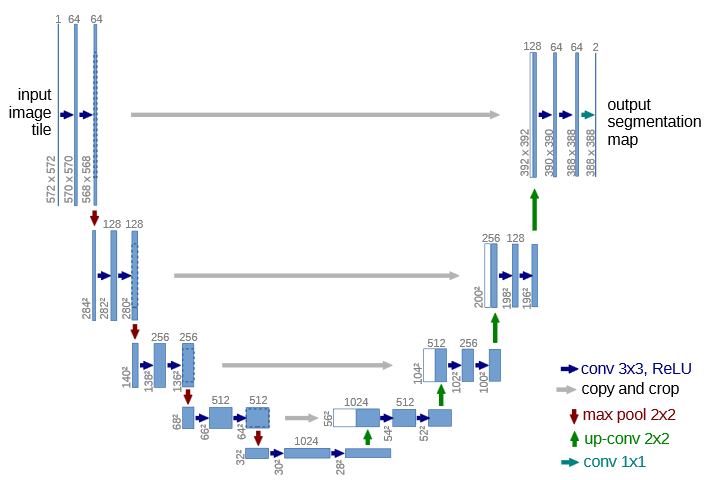
\includegraphics[width=0.8\linewidth]{../pics/UNet_Biomedical}
    \caption{The image is taken from the university of Freiburg~\cite{ronneberger2015u}}
\end{figure}



\section*{Pipeline}

\begin{figure}[ht]
    \centering
    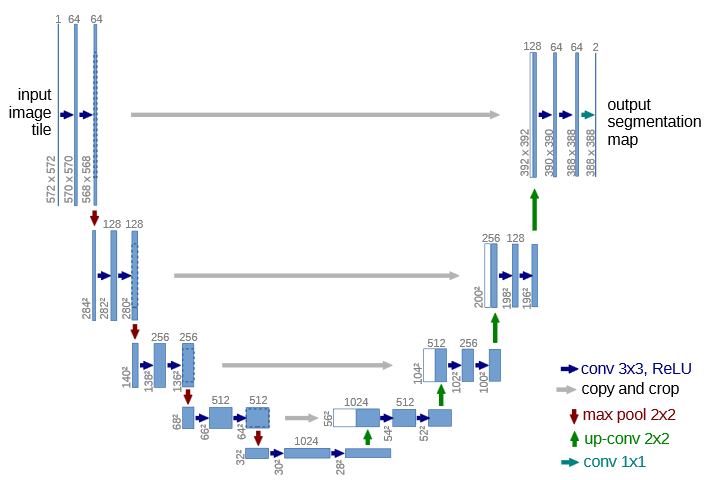
\includegraphics[width=0.8\linewidth]{../pics/UNet_Biomedical}
    \caption{The image is taken from the university of Freiburg~\cite{ronneberger2015u}}
\end{figure}



\begin{figure}[ht]
    \centering
    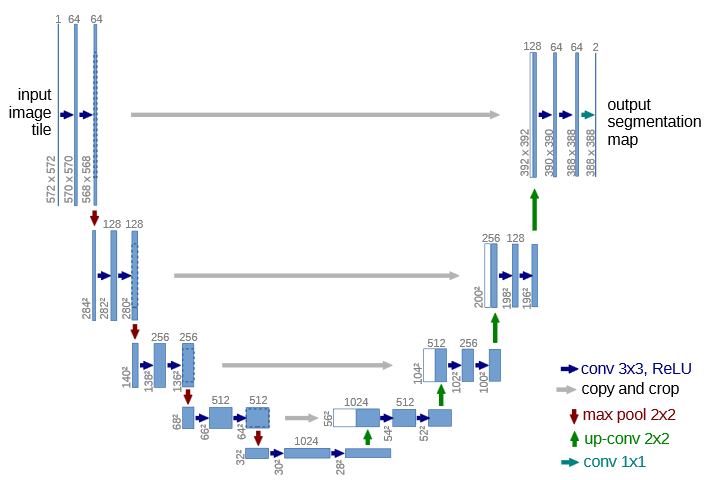
\includegraphics[width=0.8\linewidth]{../pics/UNet_Biomedical}
    \caption{The image is taken from the university of Freiburg~\cite{ronneberger2015u}}
\end{figure}

\section*{Conclusion and Future Work}


\end{document}

